%==========================================
%
% SIBGRAPI 2024 paper template
% Castelo da Vânia -- Documentação Etapa 2
%
%==========================================

\documentclass[10pt,conference]{IEEEtran}

\usepackage{cite}

\ifCLASSINFOpdf
   \usepackage[pdftex]{graphicx}
   \graphicspath{{figs/}}
   \DeclareGraphicsExtensions{.pdf,.jpeg,.png}
\else
   \usepackage[dvips]{graphicx}
   \graphicspath{{../figs/}}
   \DeclareGraphicsExtensions{.eps}
\fi

\usepackage[cmex10]{amsmath}
\interdisplaylinepenalty=2500
\usepackage{amsthm}
\newtheorem{definition}{Definition}

\usepackage{algorithmic}
\usepackage{array}

\ifCLASSOPTIONcompsoc
  \usepackage[caption=false,font=normalsize,labelfont=sf,textfont=sf]{subfig}
\else
  \usepackage[caption=false,font=footnotesize]{subfig}
\fi

\usepackage{url}
\usepackage[utf8]{inputenc}
\usepackage[T1]{fontenc}

\hyphenation{op-tical net-works semi-conduc-tor}

%------------------------------------------------- 
\newif\iffinal
\finaltrue
%\finalfalse
\newcommand{\cmtid}{99999}
%------------------------------------------------- 

\iffinal
\else
\usepackage[switch]{lineno}
\fi

\begin{document}

\title{Castelo da Vânia: Documentação do Projeto}

\iffinal

\author{
\IEEEauthorblockN{Alicia Silva Nascimento \\ Bruna de Andrade da Silva \\ Bruna Luísa Costa Reis dos Santos \\ Maria Eduarda Oliveira de A}
}

\else
  \author{SIBGRAPI Paper ID: \cmtid \\ }
  \linenumbers
\fi

\maketitle

\begin{abstract}
Este documento descreve o projeto \textit{Castelo da Vânia}, um jogo de plataforma 2.5D desenvolvido na engine Godot 4.6 para a disciplina de Computação Gráfica. O jogo situa-se em uma ambientação de horror gótico na Transilvânia, onde a protagonista Vânia deve defender seu castelo de um invasor do futuro. Esta documentação cobre a proposta geral do jogo, mecânicas de luz e sombra, recursos gráficos extras, funções de câmera, estrutura das três fases e as principais inspirações criativas e visuais do projeto.
\end{abstract}

\IEEEpeerreviewmaketitle


% ------------------------------------------------
\section{Introdução e Proposta Geral}

\textit{Castelo da Vânia} é um jogo do gênero plataforma com perspectiva 2.5D (3D com câmera fixa em um dos eixos), desenvolvido na engine Godot 4.6 para PC. O projeto aplica de forma prática conceitos de Computação Gráfica, com ênfase em iluminação, sombras e uso funcional de câmera, integrados diretamente à jogabilidade.

A proposta une estética gótica e tecnológica em uma narrativa de horror geracional. A protagonista, Vânia, deve enfrentar um invasor do futuro que ameaça tomar controle do castelo durante a Lua de Sangue.

% ------------------------------------------------
\section{História}

No coração da Transilvânia, em um mundo que une o gótico e o tecnológico, ergue-se uma lenda que atravessa séculos. O jogo \textit{Castelo da Vânia} mergulha o jogador em uma narrativa de horror gótico e dever ancestral, focando na luta da personagem principal, Vânia, contra o despertar do mal absoluto nos corredores de seu lar.

Quando a Lua de Sangue tinge o céu da Transilvânia, o véu entre as eras se rompe. Do amanhã, surge o pior pesadelo de sua linhagem: um antigo inimigo da família que viaja no tempo com um exército aliado para roubar o controle do castelo.

Vânia tem até o amanhecer para selá-lo de volta ao futuro, antes que ele finque suas raízes neste mundo e se torne forte demais para ser detido. O selamento é apenas uma solução temporária: se ela for capaz de derrota-lo de vez, encerrará para sempre um ciclo de dor que já assombra sua família há gerações.

% ------------------------------------------------
\section{Protagonista}

\subsection{Vânia}

A protagonista é Vânia, guardiã do castelo e última representante de sua linhagem. Ela carrega o peso de uma maldição geracional e deve enfrentar o invasor que ameaça seu lar usando habilidades herdadas de sua família.

\begin{figure}[!t]
\centering
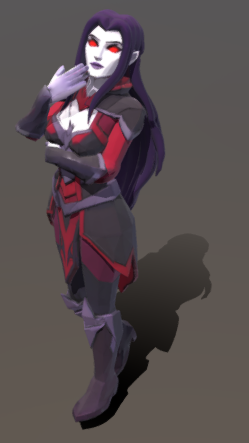
\includegraphics[width=1.4in]{img_p4_3.png}
\caption{Modelo 3D da protagonista Vânia.}
\label{fig_vania}
\end{figure}

% ------------------------------------------------
\section{Inspirações}

\subsection{Castlevania}

O jogo é fortemente inspirado nas mecânicas e visual dos primeiros cinco jogos da franquia principal de \textit{Castlevania}, tendo como base também a temática de maldição geracional e a ideia de invasão ao castelo invertida -- aqui, é a protagonista quem defende o castelo, e não quem o invade.

\begin{figure}[!t]
\centering
\subfloat[Cena de diálogo clássico]{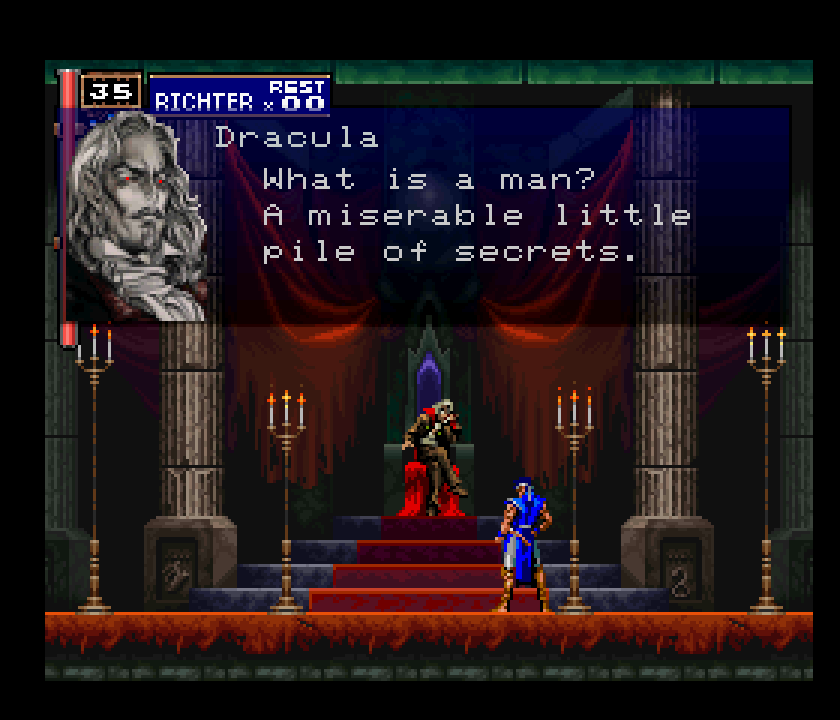
\includegraphics[width=1.5in]{img_p2_1.png}\label{fig_cv1}}
\hfil
\subfloat[Gameplay lateral 2.5D]{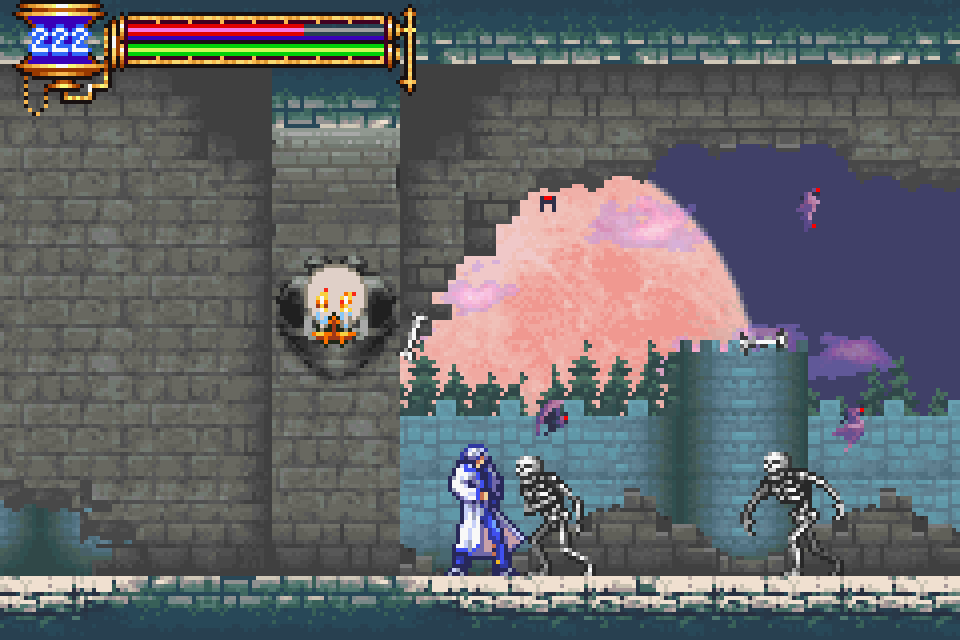
\includegraphics[width=1.5in]{img_p2_2.png}\label{fig_cv2}}
\caption{Referências visuais e de jogabilidade da franquia \textit{Castlevania}.}
\label{fig_castlevania}
\end{figure}

\begin{figure}[!t]
\centering
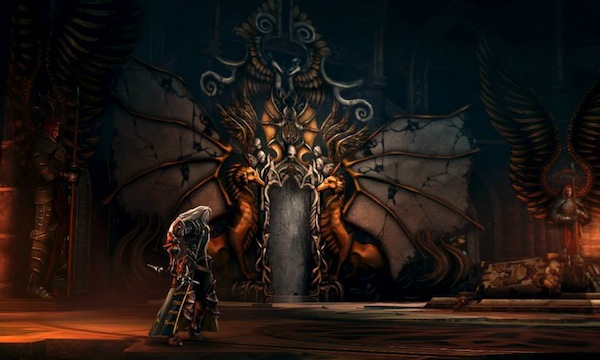
\includegraphics[width=2.0in]{img_p2_3.png}
\caption{Referência de boss design da franquia \textit{Castlevania}.}
\label{fig_cv_boss}
\end{figure}

\subsection{Hora de Aventura}

Parte da estética e dos elementos de cenário é baseada no universo de \textit{Hora de Aventura}, especificamente na personagem Marceline, a Rainha Vampiro. O foco é utilizar seu marcante Baixo-Machado como uma referência visual integrada ao ambiente do castelo.

\begin{figure}[!t]
\centering
\subfloat[Baixo-Machado]{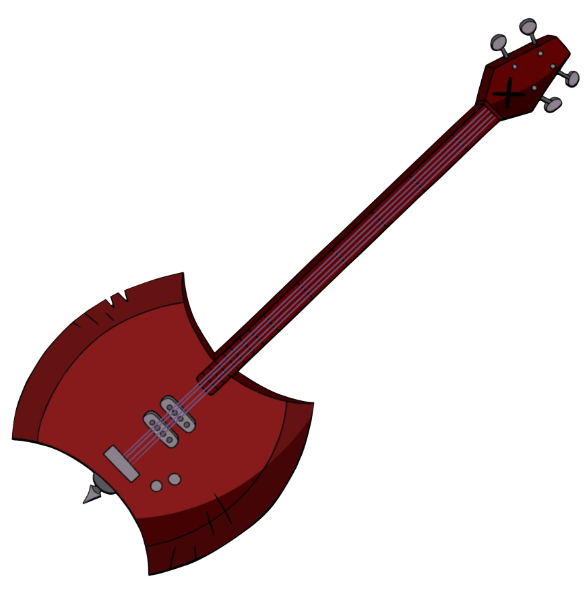
\includegraphics[width=0.9in]{img_p3_1.png}\label{fig_axebass}}
\hfil
\subfloat[Marceline, a Rainha Vampiro]{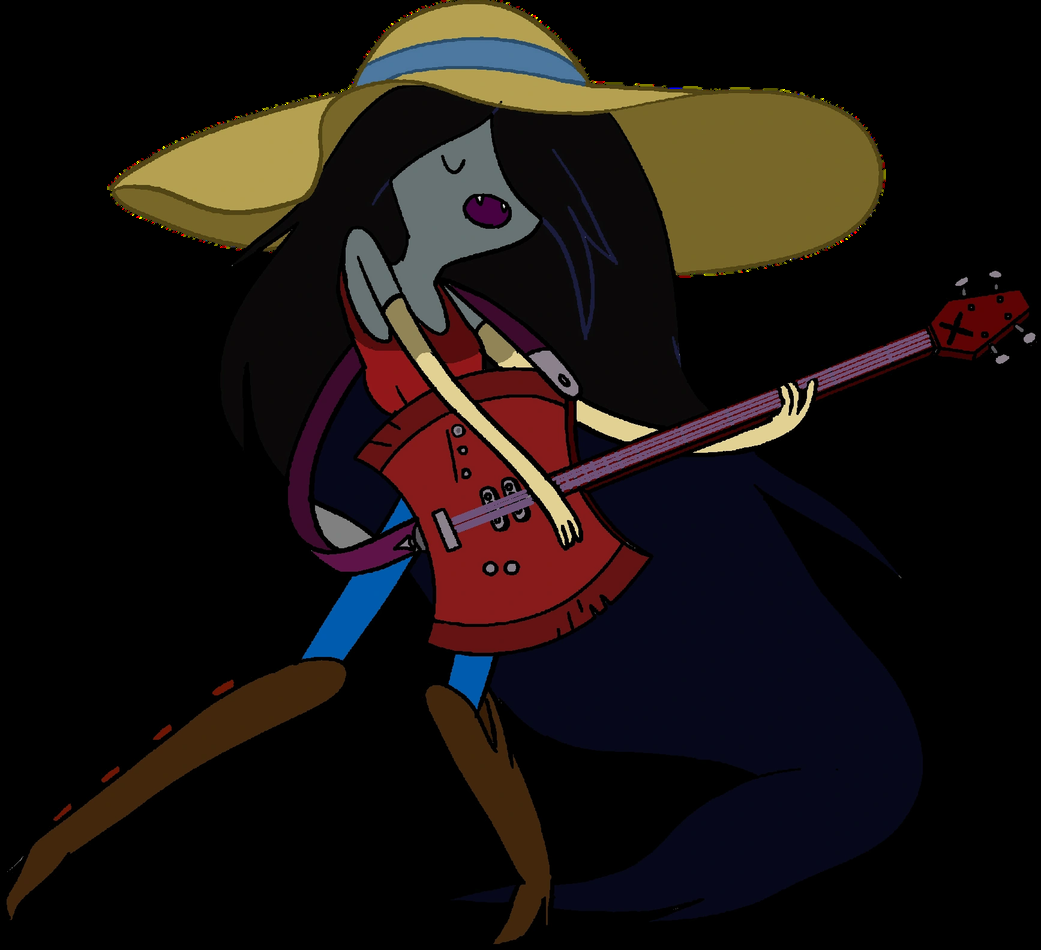
\includegraphics[width=1.6in]{img_p3_2.png}\label{fig_marceline}}
\caption{Referência estética: Marceline de \textit{Hora de Aventura}.}
\label{fig_aventura}
\end{figure}

\subsection{Pokémon}

Parte dos conceitos tecnológicos e dos poderes do Boss é inspirada no Pokémon \textit{Iron Bundle}, versão paradox de \textit{Delibird}. Ambos possuem a habilidade \textit{Present}, na qual o Pokémon lança um presente contra o inimigo sem saber o efeito -- podendo causar dano, curar, finalizar ou não ter efeito algum, como uma espécie de roleta russa.

\begin{figure}[!t]
\centering
\subfloat[Delibird]{
\includegraphics[width=1.1in]{img_p4_1.png}\label{fig_delibird}}
\hfil
\subfloat[Iron Bundle]{
\includegraphics[width=1.1in]{img_p4_2.png}\label{fig_ironbundle}}
\caption{Referência de habilidades do Boss: \textit{Delibird} e \textit{Iron Bundle}.}
\label{fig_pokemon}
\end{figure}

% ------------------------------------------------
\section{Jogabilidade Base (Plataforma 2.5D)}

O jogo implementa os requisitos base de jogabilidade de plataforma:

\begin{itemize}
    \item Movimentação horizontal do personagem;
    \item Salto;
    \item Colisão funcional com cenário e obstáculos;
    \item Elementos de risco, desafio e progressão;
    \item Condição de avanço entre fases.
\end{itemize}

A perspectiva 2.5D é mantida por meio de câmera fixa em um eixo sobre cenas construídas em 3D, preservando a profundidade visual do ambiente gótico.

% ------------------------------------------------
\section{Mecânica Principal: Luz e Sombra}

A mecânica central do jogo baseia-se na \textbf{visibilidade condicionada pela iluminação}. Na Fase 2, o castelo está dominado pela escuridão, e a protagonista possui visão reduzida. O jogador precisa explorar o ambiente e descobrir mecânicas para acender as luzes, revelando progressivamente o cenário, caminhos e obstáculos.

Essa mecânica interfere diretamente na experiência do jogador: sem luz, áreas do mapa ficam inacessíveis ou perigosas, e certas interações só são possíveis sob iluminação adequada. A luz, portanto, é tanto elemento narrativo quanto componente funcional da jogabilidade.

% ------------------------------------------------
\section{Fases}

\subsection{Fase 1 -- Exterior do Castelo}

A fase se inicia na área exterior, na entrada do castelo principal. Vânia se encaminha para o castelo e precisa enfrentar os inimigos presentes: os corvos robóticos. O ambiente conta com névoa e iluminação noturna da Lua de Sangue.

\begin{figure}[!t]
\centering
\subfloat[Corvo robótico (frente)]{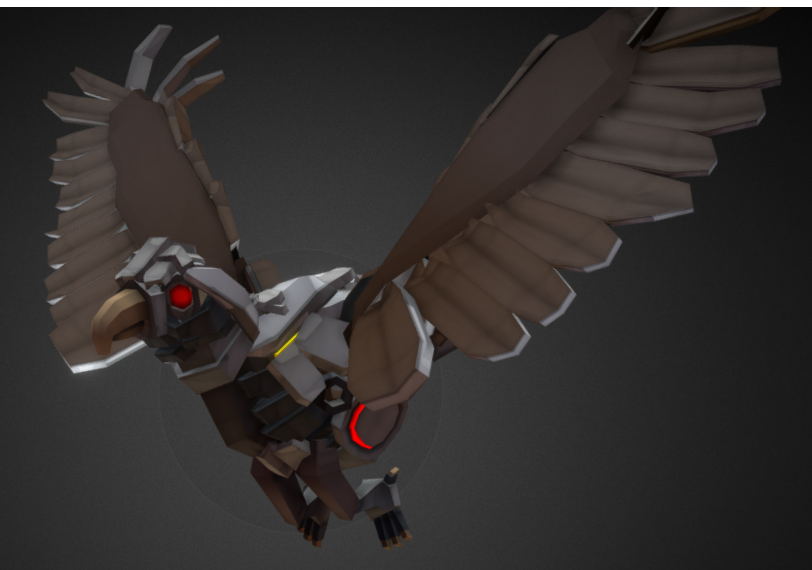
\includegraphics[width=1.5in]{img_p5_1.png}\label{fig_crow1}}
\hfil
\subfloat[Corvo robótico (lateral)]{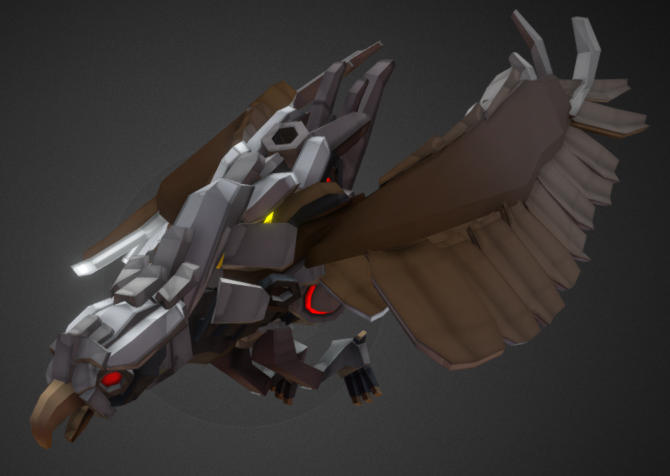
\includegraphics[width=1.5in]{img_p5_2.png}\label{fig_crow2}}
\caption{Inimigos da Fase 1: corvos robóticos.}
\label{fig_corvos}
\end{figure}

\subsection{Fase 2 -- Interior Escuro do Castelo}

Começa na entrada do castelo, dominada pela escuridão. A mecânica principal de luz e sombra é introduzida aqui: a protagonista deve desvendar mecânicas com visão reduzida e, ao final, consegue acender as luzes, revelando o ambiente e desbloqueando progressão.

\subsection{Fase 3 -- Profundezas do Castelo e Boss}

Avançando nas profundezas do castelo, agora com o auxílio das luzes restabelecidas, Vânia busca a chave que destrava a passagem até o invasor do castelo. Esta fase culmina no confronto com o Boss Final.

% ------------------------------------------------
\section{Recursos Gráficos Extras}

O projeto implementa ao menos três recursos gráficos extras além da mecânica principal de luz e sombra:

\begin{enumerate}
    \item \textbf{Partículas:} presentes nos itens encontrados na Fase 2, contribuindo para a leitura visual de objetos interativos.
    \item \textbf{Névoa (\textit{Fog}):} presente no exterior do castelo (Fase 1), reforçando a atmosfera gótica e a profundidade da cena.
    \item \textbf{Efeitos visuais de dano e interação:} efeitos perceptíveis em todas as fases, indicando ao jogador eventos de impacto, checkpoint e interação com o cenário.
\end{enumerate}

% ------------------------------------------------
\section{Uso de Câmera}

O projeto implementa ao menos duas funções de câmera além do acompanhamento básico do personagem:

\begin{enumerate}
    \item \textbf{Zoom no Boss Final (Fase 3):} ao entrar na área do Boss, a câmera realiza um zoom dramático para evidenciar o confronto e criar tensão narrativa.
    \item \textbf{Zoom dinâmico durante a gameplay:} a câmera ajusta seu zoom de forma dinâmica em momentos específicos, melhorando a leitura espacial e destacando eventos relevantes para o jogador.
\end{enumerate}

% ------------------------------------------------
\section{Entregas}
\subsection{ Etapa 1 — Protótipo Técnico}
Na primeira etapa do projeto, o grupo concluiu todos os itens exigidos para o protótipo técnico. Foi implementada a movimentação horizontal da protagonista Vânia e o sistema de salto, ambos com colisão básica funcional com o cenário. A câmera inicial foi configurada com acompanhamento do personagem, e um bloco jogável preliminar foi disponibilizado para validação das mecânicas base.

Além da jogabilidade fundamental, o grupo apresentou a proposta da mecânica principal baseada em luz e sombra — centrada na visão reduzida da protagonista na Fase 2 e na necessidade de acender as luzes para progredir. O planejamento das três fases também foi definido nesta etapa: exterior do castelo (Fase 1), interior escuro (Fase 2) e profundezas com Boss (Fase 3). Por fim, foram indicados preliminarmente os recursos gráficos extras (partículas, névoa e efeitos de dano) e as funções de câmera (zoom no Boss e zoom dinâmico) que seriam implementados nas etapas seguintes.

\subsection{ Etapa 2 — Vertical Slice}
\subsubsection{Mecânica de Luz e Sombra}
Optamos por utilizar um efeito de aura vermelha, para dar o efeito de iluminação noturna da Lua de Sangue, que é uma peça importante na história do jogo.

\begin{figure}[h]
\centering
\subfloat[Screenshot do jogo]{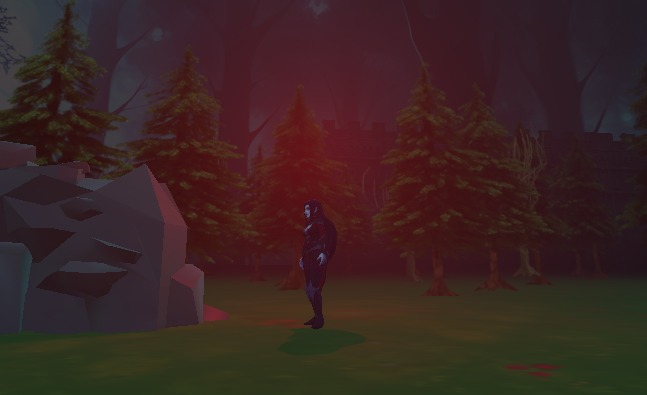
\includegraphics[width=3.1in]{vania-luz.png}\label{figvanialuz}}
\caption{Mecânica de luz}
\label{fig_luz}
\end{figure}

\subsubsection{Obstáculos}
Durante a \textit{gameplay}, um dos principais desafios é avançar no mapa. Pulando plataformas, evitando espinhos e inimigos, os corvos, que surgem pelo caminho.

\begin{figure}[!h]
\centering
\subfloat[Plataformas e Espinhos]{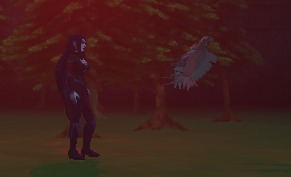
\includegraphics[width=3.1in]{vania-corvo.jpg}\label{fig_espinhos}}
\hfil
\subfloat[Inimigos - Corvos Robóticos]{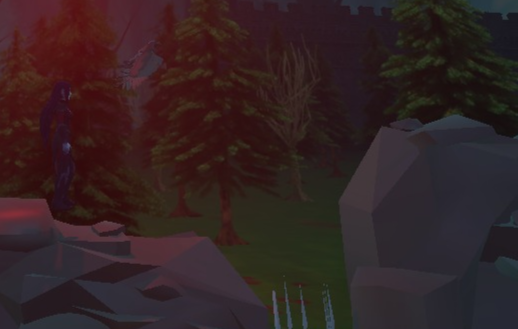
\includegraphics[width=3.1in]{vania-espinhos.png}\label{fig_corvo}}
\caption{Screenshot do jogo demonstrando obstáculos e inimigos}
\label{fig_obstaculos}
\end{figure}

\subsubsection{Itens}
Durante o jogo, o jogador terá a possibilidade de coletar itens essenciais para sua progressão. Introduzimos na Etapa 2 o \textbf{Suco de Morango}, um item de cura que restaura 20\% da vida total da personagem.

A escolha de um item consumível em vez de sangue como fonte de energia possui uma justificativa na narrativa:

\begin{itemize}
    \item \textbf{Habilidade de Absorção:} Assim como a personagem Marceline, de \textit{Hora de Aventura}, a protagonista Vânia possui a habilidade de extrair a cor vermelha de objetos, pessoas e alimentos. Então, ao consumir o ``vermelho'' do suco, ela recupera 20 pontos de vida.
    
    \item \textbf{Tom do Jogo:} Optamos por essa abordagem para evitar elementos excessivamente \textit{gore} (gráficos ou violentos), permitindo que a narrativa mantenha uma atmosfera mais equilibrada, sem recorrer à temática de sangue explícito.
\end{itemize}

\begin{figure}[h]
\centering
\subfloat[Screenshot do item Suco de Morango]{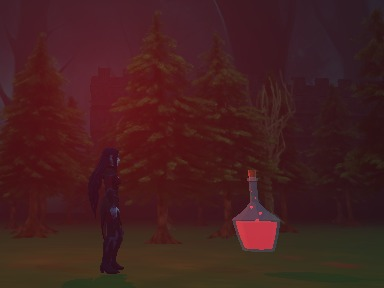
\includegraphics[width=2.0in]{vania-suco.jpg}\label{fig_suco}}
\end{figure}

% ------------------------------------------------
\section*{Referências de Assets}

\begin{itemize}
    \item Árvores e objetos LP: \url{https://sketchfab.com/3d-models/lp-objects-trees-8b9e6a7e72914f668f4762f7723167f9}
    \item Personagem feminina vampira: \url{https://sketchfab.com/3d-models/vampire-female-1164848e02bc463ab2305b94c1818cd6}
    \item Mike, o pássaro (animações): \url{https://sketchfab.com/3d-models/mike-the-bird-all-animations-583211a5935449ab92179aed53b2f4f2}
\end{itemize}

\end{document}
